\section{Experimental Results}
\label{sec:experiments}

We evaluate both traditional methods and deep learning approaches—under fine-tuning and training-from-scratch regimes—on a 1{,}000-species subsample of mini-iNat2021. Additionally, we conduct ablation studies on input features, hyperparameters, data augmentations, and regularization techniques.

%-------------------------------------------------------------------------
\subsection{Experimental setup}
\label{sec:exp-setup}

\paragraph{Dataset.}
We construct a 1{,}000-species subsample of mini-iNat2021 containing 50 images per class, totaling 50,000 images. For each class, 40 images are used for training and 10 images are used for validation (an 80\%/20\% train/validation split). An additional 10,000 unseen images are reserved exclusively for testing.

\paragraph{Metrics.}
We report balanced accuracy, Top-1 accuracy, Top-5 accuracy, and macro-averaged precision, recall, and F1 score.

\paragraph{Reproducibility.}
All experiments are conducted using the fixed random seed \texttt{20269517}.

%-------------------------------------------------------------------------
\subsection{Traditional Methods}
\label{sec:trad-methods}

\subsubsection{Random Forests}
\label{sec:trad-rf}

\paragraph{Feature Extraction}
\label{sec:feat-extract}
Images are resized to dim (128, 128) before being passed into colour histogram and HOG feature extraction functions. A baseline feature space was first created (first rows of \cref{tab:colour-hist-config}
and \cref{tab:hog-config}), followed by ablation studies that adjusted the colour space individually to L*a*b for the colour histograms while retaining the same HOG configuration as the base, and another
study that adjusted the number of cell pixels for the HOG features while retaining the HSV colour space for the colour histograms. The configurations for both of these studies are shown in
\cref{tab:colour-hist-config} and \cref{tab:hog-config}.

\begin{table}[h]
  \centering
  \small
  \caption{Colour histogram configuration.}
  \label{tab:colour-hist-config}
  \begin{tabular}{@{}lll@{}}
    \toprule
    Colour Space & Bins per Channel      & Value Range                \\
    \midrule
    HSV          & $8 \times 8 \times 8$ & H: [0, 180], S/V: [0, 256] \\
    L*a*b        & $8 \times 8 \times 8$ & [0, 256] (all channels)    \\
    \bottomrule
  \end{tabular}
\end{table}

\begin{table}[h]
  \centering
  \small
  \caption{HOG configuration.}
  \label{tab:hog-config}
  \begin{tabular}{@{}llll@{}}
    \toprule
    Stage    & Orientation & Cell Pixels  & Block Cells  \\
    \midrule
    Base     & 9           & $8 \times 8$ & $2 \times 2$ \\
    Ablation & 9           & $6 \times 6$ & $2 \times 2$ \\
    \bottomrule
  \end{tabular}
\end{table}

\paragraph{Modelling and Training}
\label{sec:model-and-train-rf}
Each of these feature spaces was separately fed into a random forest classifier with \texttt{n\_estimators=150, max\_depth=20, n\_jobs=-1, warm\_start=True, random\_state=20269517}. The accuracy, precision,
recall and F1 score for these are reported in \cref{tab:rf-feature-comparison}.

\begin{table*}[t]
  \centering
  \small
  \caption{Validation results for Random Forest feature configurations.}
  \label{tab:rf-feature-comparison}
  \begin{tabular}{@{}lrrrrrrr@{}}
    \toprule
    Model                   & Train Time (min) & (Bal.) Acc.     & Top-1 Acc.      & Top-5 Acc.      & Prec. (macro)   & Recall (macro)  & F1 (macro)      \\
    \midrule
    Baseline (HSV, HOG 8x8) & 191.8            & \textbf{0.0319} & \textbf{0.0319} & \textbf{0.0999} & \textbf{0.0191} & \textbf{0.0319} & \textbf{0.0186} \\
    HOG diff (cells 6x6)    & 246.7            & 0.0281          & 0.0281          & 0.0880          & 0.0127          & 0.0281          & 0.0150          \\
    LAB colour space        & 185.1            & 0.0279          & 0.0279          & 0.0928          & 0.0157          & 0.0279          & 0.0158          \\
    \bottomrule
  \end{tabular}
\end{table*}

From this, since mini-iNat2021 contains fine-grained images, putting more emphasis on the F1 score results in the baseline being the best model to move forward with. Using this baseline model, further training was
carried out with \texttt{n\_estimator} values of 200, 300, and 400 to see if more training improved accuracy. The results are shown in \cref{tab:rf-longer-training}.

\begin{table*}[t]
  \centering
  \small
  \caption{Validation results for baseline model trained with additional estimators.}
  \label{tab:rf-longer-training}
  \begin{tabular}{@{}lrrrrrrr@{}}
    \toprule
    Model                     & Add. Train Time (min) & (Bal.) Acc.     & Top-1 Acc.      & Top-5 Acc.      & Prec. (macro)   & Recall (macro)  & F1 (macro)      \\
    \midrule
    Baseline (200 estimators) & 64.9                  & 0.0340          & 0.0340          & 0.1014          & 0.0207          & 0.0340          & 0.0201          \\
    Baseline (300 estimators) & 129.4                 & 0.0358          & 0.0358          & 0.1087          & 0.0204          & 0.0358          & 0.0209          \\
    Baseline (400 estimators) & 126.5                 & \textbf{0.0395} & \textbf{0.0395} & \textbf{0.1131} & \textbf{0.0243} & \textbf{0.0395} & \textbf{0.0231} \\
    \bottomrule
  \end{tabular}
\end{table*}

From this, it can be seen that additional estimators provide only marginal improvement, with the model at 400 estimators achieving the best validation F1 score. However, when evaluated on the test set, the
model with 300 estimators achieved the best F1 score (recorded in \cref{tab:overall-comparison}), narrowly outperforming the 400-estimator model despite the latter's slightly higher validation performance.
Given that the difference between the 300- and 400-estimator models is minimal on both validation and test sets (accuracy and F1 differing by only 0.0004), this discrepancy is more likely due to the inherent
randomness of Random Forest's bootstrap sampling than to genuine overfitting, indicating that performance has effectively started to plateau from approximately 300 estimators.

\paragraph{Error Analysis}
\label{sec:rf-error-analysis}
Because the model trained with 300 estimators achieved the best macro-F1 score on the test data, it was selected for the remaining error analysis. First, the top 20 most confused species pairs were identified 
and visualised as a confusion matrix (spanning 30+ species classes in total; \cref{fig:top20_confused} in the supplementary material). This revealed that most confusion arises within insects and arthropods (\textit{Arthropoda}), vertebrates 
(\textit{Chordata}), sac fungi (\textit{Ascomycota}), and vascular plants (\textit{Tracheophyta}). A phylum-level confusion matrix (\cref{fig:cm_phylum_level} in the supplementary material) clarified this further, showing substantial 
misclassification of arthropods (\textit{Arthropoda}) as vascular plants (\textit{Tracheophyta}), and of vertebrates (\textit{Chordata}) as both arthropods (\textit{Arthropoda}) and vascular plants 
(\textit{Tracheophyta}). This may be partly explained by the fact that insects are frequently photographed while resting on or camouflaged among plants, causing the model to pick up on background vegetation 
rather than the insect's own distinguishing features.

\subsubsection{BoVW--RootSIFT with Linear SVM}
\label{sec:trad-svm}
 
\textbf{Experimental setup.}
Following \cref{sec:exp-setup}, development uses 40 training and 10 validation images per species, with 10 held-out test images per species for final evaluation. Vocabulary construction, representation selection, and $C$ tuning use only the training and validation splits.
 
\emph{Features.} Each image is resized so its longer side is 256\,px and converted to greyscale. Sparse SIFT keypoints are detected, their descriptors converted to RootSIFT, and images with more than 500 descriptors keep the 500 strongest by keypoint response. Descriptors are extracted once and cached, so all variants share identical local features.
 
\emph{Vocabulary and encoding.} The vocabulary is learned from training descriptors only, using mini-batch $k$-means (batch size 10{,}000, three initialisations, 100 iterations) on up to 500{,}000 sampled descriptors, with 1{,}024 words in the baseline. The baseline uses hard assignment, TF-IDF weighting, no spatial pyramid, and L2 normalisation. Soft assignment instead spreads each descriptor over its five nearest words with Gaussian weights whose bandwidth is the median training-descriptor-to-centre distance. The Spatial Pyramid Matching (SPM) variant concatenates one global histogram with four from a $2\times2$ grid (global weight 0.5, cells sharing the rest, then L2 normalisation), expanding the 1{,}024-word representation to 5{,}120 dimensions.
 
\emph{Protocol.} Individual ablations use a linear SVM with $C=1$ and sweep $K\in\{256,512,1024,2048\}$, then soft assignment, TF-IDF removal, and SPM in isolation. Components that raise validation macro-F1 are combined at $K\in\{256,1024\}$, and $C\in\{10^{-4},\dots,10^{2}\}$ is finally searched separately for the baseline and the selected representation, which are frozen before test evaluation.
 
\textbf{Individual representation ablation.}
\cref{tab:svm-ablation} reports the individual experiments. Soft assignment is by far the strongest single change, raising macro-F1 from 2.62\% to 3.96\% and confirming that hard assignment introduces substantial quantisation error on this fine-grained task. SPM helps less (2.92\%), so coarse spatial layout carries only a weak signal, and removing TF-IDF is essentially neutral (2.66\%). Vocabulary size shows clear diminishing returns above 1{,}024 words, while shrinking it to 512 or 256 merges discriminative structures and hurts macro-F1.
 
\begin{table*}[t]
\centering
\caption{Validation results for the individual
BoVW--RootSIFT--SVM representation experiments. All configurations
use a linear SVM with $C=1$. SVM training time excludes SIFT extraction
and visual-vocabulary construction.}
\label{tab:svm-ablation}
\resizebox{\textwidth}{!}{
\begin{tabular}{lccccccccccc}
\toprule
Configuration &
$K$ &
Encoding &
TF-IDF &
SPM &
SVM Train Time (min) &
(Bal.) Acc. &
Top-1 Acc. &
Top-5 Acc. &
Prec. (macro) &
Recall (macro) &
F1 (macro) \\
\midrule
Baseline
& 1024 & Hard & Yes & No
& 10.2
& 0.0294 & 0.0294 & 0.0723
& 0.0250 & 0.0294 & 0.0262 \\
 
Vocabulary 256
& 256 & Hard & Yes & No
& 6.1
& 0.0278 & 0.0278 & 0.0752
& 0.0175 & 0.0278 & 0.0196 \\
 
Vocabulary 512
& 512 & Hard & Yes & No
& 8.1
& 0.0286 & 0.0286 & 0.0724
& 0.0218 & 0.0286 & 0.0237 \\
 
Vocabulary 2048
& 2048 & Hard & Yes & No
& 11.0
& 0.0293 & 0.0293 & 0.0717
& 0.0272 & 0.0293 & 0.0272 \\
 
Soft assignment
& 1024 & Soft & Yes & No
& 31.6
& \textbf{0.0485} & \textbf{0.0485} & \textbf{0.1107}
& \textbf{0.0368} & \textbf{0.0485} & \textbf{0.0396} \\
 
No TF-IDF
& 1024 & Hard & No & No
& 10.4
& 0.0297 & 0.0297 & 0.0718
& 0.0255 & 0.0297 & 0.0266 \\
 
Spatial pyramid
& 1024 & Hard & Yes & Yes
& 24.0
& 0.0325 & 0.0325 & 0.0764
& 0.0285 & 0.0325 & 0.0292 \\
\bottomrule
\end{tabular}
}
\end{table*}
 
\textbf{Combined representation and $C$ tuning.}
Combining the three beneficial components (\cref{tab:svm-combined}) is strongest at 1{,}024 words (macro-F1 4.26\%) and exceeds the best individual result (3.96\%), so their gains are at least partially complementary. Tuning $C$ selects $0.1$ for the baseline (2.73\%) and $1$ for the improved representation, both frozen for test evaluation.
 
\begin{table}[t]
\centering
\caption{Validation results for the combined BoVW configurations.
Both configurations use soft assignment, no TF-IDF, Spatial Pyramid
Matching, and $C=1$.}
\label{tab:svm-combined}
\resizebox{\columnwidth}{!}{
\begin{tabular}{lccccc}
\toprule
Configuration &
Vocabulary &
Feature Dim. &
Top-1 Acc. &
Top-5 Acc. &
F1 (macro) \\
\midrule
Combined-256
& 256
& 1280
& 0.0470
& 0.1069
& 0.0359 \\
 
Combined-1024
& 1024
& 5120
& \textbf{0.0509}
& \textbf{0.1144}
& \textbf{0.0426} \\
\bottomrule
\end{tabular}
}
\end{table}
 
\textbf{Held-out test results.}
On the held-out test set (\cref{tab:svm-test}), the improved representation raises macro-F1 from 2.65\% to 4.26\% and Top-1 from 3.63\% to 5.14\% over the tuned baseline, and its test macro-F1 matches validation (4.26\%), so the selection transfers without over-fitting. This gain is costly: soft assignment and the 5{,}120-dimensional SPM features raise SVM training from 9.0 to 90.4\,min and test encoding from 11.7 to 142.6\,s. Even so, absolute performance stays low for 1{,}000-way fine-grained recognition, as visual-word histograms remain far less expressive than the learned deep features of \cref{sec:dl-methods}.
 
\begin{table*}[t]
\centering
\caption{Held-out test results for the frozen baseline and selected
improved BoVW--RootSIFT--SVM configurations.}
\label{tab:svm-test}
\resizebox{\textwidth}{!}{
\begin{tabular}{lcccccccc}
\toprule
Configuration &
SVM Train Time (min) &
Test Encoding Time (s) &
(Bal.) Acc. &
Top-1 Acc. &
Top-5 Acc. &
Prec. (macro) &
Recall (macro) &
F1 (macro) \\
\midrule
Baseline BoVW
& 9.0
& 11.69
& 0.0363
& 0.0363
& 0.0921
& 0.0243
& 0.0363
& 0.0265 \\
 
Improved BoVW
& 90.4
& 142.59
& \textbf{0.0514}
& \textbf{0.0514}
& \textbf{0.1163}
& \textbf{0.0397}
& \textbf{0.0514}
& \textbf{0.0426} \\
\bottomrule
\end{tabular}
}
\end{table*}
 
\paragraph{Error analysis.}
The row-normalised confusion matrix over all 1{,}000 classes (\cref{fig:suppl-svm-confusion-full} in the supplementary material) shows a faint diagonal against a diffuse background of errors, consistent with the low but above-chance accuracy: most images are misclassified and errors are spread widely rather than concentrated. Since the full matrix is dominated by this diffuse mass, we inspect the most-confused species subset (\cref{fig:suppl-svm-confusion-subset}), which exposes clear structure. The strongest confusions fall between visually and taxonomically similar species: among cobweb spiders, \textit{Steatoda grossa} is frequently predicted as \textit{Eratigena duellica}; among seabirds and waterfowl with similar dark plumage, \textit{Bucephala albeola}, \textit{Melanitta deglandi}, and \textit{Cerorhinca monocerata} are mutually confused; and pairs such as \textit{Platanthera bifolia} with \textit{Etlingera elatior} follow the same pattern. This indicates that the BoVW--RootSIFT histogram captures coarse colour and shape cues well enough to group organisms of broadly similar appearance, but lacks the discriminative power to separate species differing only in subtle local detail, the limitation motivating the deep representations of \cref{sec:dl-methods}. A few classes such as \textit{Ardenna creatopus} retain a strong diagonal, showing the pipeline succeeds where inter-class differences are relatively large.

%-------------------------------------------------------------------------
\subsection{Deep Learning Methods}
\label{sec:dl-methods}

\subsubsection{EfficientNet V2}
\label{sec:dl-efficientnetv2}

\paragraph{Experimental setup.}
We train TorchVision EfficientNetV2-S on $384\times384$ inputs and replace its final layer with a $1{,}280$-to-$1{,}000$ species classifier. All layers remain trainable. Pretrained runs use ImageNet-1K initialization and all four cumulative augmentation levels, while scratch runs use random initialization and the None and Full endpoints. The main EfficientNet V2 training settings for the pretrained and from-scratch regimes are summarized in \cref{tab:efficientnetv2-hyperparams} in the supplementary material.

\paragraph{Main results.}
\cref{tab:efficientnetv2-results} compares four cumulative augmentation levels for the pretrained model and two endpoints for the scratch model. Every class has exactly 10 test images, so balanced accuracy (macro recall) is identical to Top-1 accuracy and is not listed separately. C (pretrained Crop+Flip) records the highest test Top-1 and macro F1 at $79.20\%$ and $79.08\%$, respectively.

\begin{table*}[t]
  \centering
  \caption{EfficientNetV2-S ablation results on the mini-iNat2021 test set. Train and test times are H:MM:SS.}
  \label{tab:efficientnetv2-results}
  \setlength{\tabcolsep}{2.8pt}
  \scriptsize
  \begin{tabular}{@{}cllcccrrrrr@{}}
    \toprule
    ID & Init       & Augmentation           & Train Time & Test Time & Epochs & Top-1 Acc.      & Top-5 Acc.      & Prec. (macro)   & Recall (macro)  & F1 (macro)      \\
    \midrule
    A  & Pretrained & None                   & 3:04:17    & 0:02:02   & 30     & 0.7763          & 0.9226          & 0.7909          & 0.7763          & 0.7742          \\
    B  & Pretrained & Crop                   & 3:13:57    & 0:00:53   & 30     & 0.7862          & 0.9290          & 0.8017          & 0.7862          & 0.7843          \\
    C  & Pretrained & Crop+Flip              & 3:20:39    & 0:00:53   & 30     & \textbf{0.7920} & 0.9321          & 0.8074          & \textbf{0.7920} & \textbf{0.7908} \\
    D  & Pretrained & Crop+Flip+Color Jitter & 3:29:48    & 0:00:55   & 30     & 0.7917          & \textbf{0.9325} & \textbf{0.8076} & 0.7917          & 0.7903          \\
    E  & Scratch    & None                   & 3:14:53    & 0:00:54   & 30     & 0.3188          & 0.5492          & 0.3474          & 0.3188          & 0.3156          \\
    F  & Scratch    & Crop+Flip+Color Jitter & 5:31:07    & 0:00:54   & 50     & 0.4852          & 0.7055          & 0.4998          & 0.4852          & 0.4807          \\
    \bottomrule
  \end{tabular}
\end{table*}

\paragraph{Transfer learning vs.\ training from scratch.}
Without augmentation, pretraining raises Top-1 from $31.88\%$ (E) to $77.63\%$ (A), a $45.75$-point gain. With full augmentation, it raises Top-1 from $48.52\%$ (F) to $79.17\%$ (D), a $30.65$-point gain. Equivalently, removing transfer learning reduces Top-1 by $45.75$ and $30.65$ points in the two matched settings.

\paragraph{Effect of data augmentation.}
In the pretrained augmentation ablation, Crop raises Top-1 from $77.63\%$ to $78.62\%$ ($+0.99$ points), and Flip further raises it to $79.20\%$ ($+0.58$). Adding Color Jitter changes Top-1 to $79.17\%$ ($-0.03$), so C records the highest test Top-1. For scratch training, full augmentation raises Top-1 from $31.88\%$ to $48.52\%$ ($+16.64$) and macro F1 from $31.56\%$ to $48.07\%$ ($+16.51$). Ablating Crop or Flip reduces pretrained accuracy, whereas ablating Color Jitter increases it by $0.03$ points. Removing the full augmentation pipeline lowers Top-1 for both pretrained ($79.17\%\to77.63\%$) and scratch ($48.52\%\to31.88\%$) training.

\paragraph{Training process dynamics.}
\label{sec:dl-efficientnetv2-training-dynamics}
All six runs reach stable validation metrics within their epoch budgets and display sufficient convergence in the training curves, with some runs showing overfitting as training loss continues to fall after validation performance plateaus. For the representative Crop+Flip run, validation loss falls from $3.174$ at epoch 5 to $1.848$ at epoch 29 and ends at $1.850$, while validation Top-1 varies by only $0.19$ percentage points over epochs 25--30. The curves for all six runs are provided in \cref{fig:suppl-efficientnetv2-loss} in the supplementary material.

\paragraph{Phylum-level error analysis.}
\label{sec:dl-efficientnetv2-error-analysis}
Aggregating C's predictions by phylum gives $98.06\%$ accuracy. The two highest row-normalized error cases are both for Echinodermata: $5.00\%$ are predicted as Marchantiophyta and $5.00\%$ as Mollusca, giving a total phylum error rate of $10.00\%$ ($2/20$). Echinodermata therefore has the highest observed error percentage on this test set, based on 20 images. The count and row-normalized matrices are provided in \cref{fig:suppl-efficientnetv2-phylum} in the supplementary material.

\subsubsection{ConvNeXt V2}
\label{sec:dl-convnextv2}

\paragraph{Experimental setup.}
We train ConvNeXt V2-Tiny on $224\times224$ inputs under two initialization regimes: (i) transfer learning with ImageNet-22K-pretrained weights, fully fine-tuned end-to-end; and (ii) training from scratch with randomly initialized weights. The augmentation and regularization strategies are applied incrementally on the from-scratch regime, adding one technique at a time. The main ConvNeXt V2 training settings for the pretrained and from-scratch regimes are summarized in \cref{tab:convnextv2-hyperparams} in the supplementary material. Representative training and validation loss curves for experiments B, C, H, and I are provided in \cref{fig:suppl-convnextv2-loss} in the supplementary material. All experiments were run on a single NVIDIA T4 GPU via Google Colab.

\paragraph{Main results.}
\cref{tab:main-results} reports the ablation over initialization, cumulative augmentation level, DropPath, and warmup schedule across our $9$ experiments (A--I). B (pretrained Basic) records the highest test Top-1 and macro F1 at $81.00\%$ and $80.97\%$, respectively.

\begin{table*}[t]
  \centering
  \caption{ConvNeXt V2 ablation results on the mini-iNat2021 test set. Train and test times are H:MM:SS.
  }
  \label{tab:main-results}
  \setlength{\tabcolsep}{2.5pt}
  \scriptsize
  \begin{tabular}{@{}clccccccrrrrr@{}}
    \toprule
    ID & Init            & Augmentation    & DropPath Rate   & Warmup Steps    & Train Time      & Test Time & Num. Epochs
       & Top-1 Acc.      & Top-5 Acc.      & Prec. (macro)   & Recall (macro)  & F1 (macro)                                \\
    \midrule
    A  & Pretrained      & None            & 0.0             & 1k              & 3:29:21         & 0:01:43   & 25
       & 0.7877          & 0.9204          & 0.8030          & 0.7877          & 0.7869                                    \\
    B  & Pretrained      & Basic           & 0.0             & 1k              & 3:41:27         & 0:01:38   & 25
       & \textbf{0.8100} & \textbf{0.9320} & \textbf{0.8244} & \textbf{0.8100} & \textbf{0.8097}                           \\
    C  & Scratch         & None            & 0.0             & 1k              & 1:59:19         & 0:01:40   & 14
       & 0.1287          & 0.2984          & 0.1479          & 0.1287          & 0.1149                                    \\
    D  & Scratch         & Basic           & 0.0             & 1k              & 7:17:35         & 0:01:40   & 50
       & 0.1975          & 0.3697          & 0.1874          & 0.1975          & 0.1860                                    \\
    E  & Scratch         & Basic           & 0.1             & 1k              & 3:17:15         & 0:01:39   & 22
       & 0.1790          & 0.3753          & 0.2071          & 0.1790          & 0.1728                                    \\
    F  & Scratch         & Basic+CD        & 0.1             & 1k              & 3:43:46         & 0:01:39   & 25
       & 0.1850          & 0.3730          & 0.2098          & 0.1850          & 0.1790                                    \\
    G  & Scratch         & Basic+CD+Mix    & 0.1             & 1k              & 8:33:00         & 0:01:39   & 58
       & 0.3332          & 0.5492          & 0.3581          & 0.3332          & 0.3254                                    \\
    H  & Scratch         & Basic+CD+Mix    & 0.1             & 10k             & 18:09:21        & 0:01:40   & 112
       & 0.3768          & 0.5886          & 0.4137          & 0.3768          & 0.3689                                    \\
    I  & Scratch         & Basic+CD+Mix    & 0.1             & 30k             & 6:51:06         & 0:01:40   & 47
       & 0.2451          & 0.4489          & 0.2734          & 0.2451          & 0.2357                                    \\
    \bottomrule
  \end{tabular}
\end{table*}

\paragraph{Transfer learning vs.\ training from scratch.}
Without augmentation, pretraining raises Top-1 from $12.87\%$ (C) to $78.77\%$ (A), a $65.90$-point gain. With Basic augmentation, it raises Top-1 from $19.75\%$ (D) to $81.00\%$ (B), a $61.25$-point gain.

\paragraph{Effect of data augmentation.}
On the pretrained regime, Basic augmentation alone (A $\to$ B) improves Top-1 from $78.77\%$ to $81.00\%$ ($+2.23$). On the from-scratch regime, the incremental ladder yields: Basic (C $\to$ D) $+6.88$ Top-1 ($12.87\% \to 19.75\%$); DropPath at rate $0.1$ (D $\to$ E) $-1.85$ ($19.75\% \to 17.90\%$); CoarseDropout (E $\to$ F) $+0.60$ ($17.90\% \to 18.50\%$); and batch-level CutMix/MixUp (F $\to$ G) $+14.82$ ($18.50\% \to 33.32\%$).

\paragraph{Effect of warmup schedule.}
With the fully-augmented from-scratch configuration held fixed, the $10$k-step warmup (H) reaches $37.68\%$ Top-1, versus $33.32\%$ Top-1 for $1$k (G) and $24.51\%$ Top-1 for $30$k (I).

\paragraph{Phylum-level error analysis.}
Aggregating B's predictions by phylum gives 97.74\% accuracy. Four major row-normalized error cases stand out: one for Ascomycota, in which 5.00\% (5/100) are predicted as Tracheophyta, and three for Echinodermata, in which 5.00\% are predicted as Basidiomycota, 5.00\% as Cnidaria, and 5.00\% as Mollusca. This gives Echinodermata a total phylum error rate of 15.00\% (3/20). Echinodermata therefore has the highest observed error percentage on this 20-image test set. The count and row-normalized confusion matrices are provided in \cref{fig:suppl-convnextv2-phylum} of the supplementary material.

%-------------------------------------------------------------------------
\subsection{Overall Comparison}
\label{sec:overall-comparison}
\cref{tab:overall-comparison} summarizes the performance across all evaluated traditional and deep learning pipelines on the mini-iNat2021 test set. Hand-crafted feature baselines struggle to scale to 1{,}000-way fine-grained species categorization, with Bag-of-Visual-Words (BoVW-RootSIFT with Linear SVM) and Random Forest achieving Top-1 accuracies of only $5.14\%$ and $3.64\%$, respectively. In contrast, modern deep learning architectures leverage learned hierarchical visual representations to achieve dramatic performance improvements: EfficientNetV2-S reaches $79.20\%$ Top-1 accuracy ($79.08\%$ macro-F1), while ConvNeXt V2-Tiny achieves the highest overall performance at $81.00\%$ Top-1 accuracy ($80.97\%$ macro-F1). This highlights the necessity of end-to-end deep learning features for complex fine-grained biological visual recognition.

\begin{table*}[t]
  \centering
  \caption{Overall comparison of all evaluated methods on the mini-iNat2021 test set.}
  \label{tab:overall-comparison}
  \setlength{\tabcolsep}{3pt}
  \scriptsize
  \resizebox{0.92\textwidth}{!}{%
    \begin{tabular}{@{}llrrrrrrrr@{}}
      \toprule
      Method                     & Family        & Train (min) & Test (min) & (Bal.) Acc.     & Top-1 Acc.      & Top-5 Acc.      & Prec.           & Recall          & F1              \\
      \midrule
      BoVW--RootSIFT--Linear SVM & Traditional   & 90.40       & 2.38       & 0.0514          & 0.0514          & 0.1163          & 0.0397          & 0.0514          & 0.0426          \\
      Random Forests (300)       & Traditional   & 386.1       & 0.9        & 0.0364          & 0.0364          & 0.1061          & 0.0239          & 0.0364          & 0.0226          \\
      EfficientNet V2            & Deep Learning & 200.65      & 0.88       & 0.7920          & 0.7920          & \textbf{0.9321} & 0.8074          & 0.7920          & 0.7908          \\
      ConvNeXt V2                & Deep Learning & 221.45      & 1.63       & \textbf{0.8100} & \textbf{0.8100} & 0.9320          & \textbf{0.8244} & \textbf{0.8100} & \textbf{0.8097} \\
      \bottomrule
    \end{tabular}%
  }
\end{table*}

%-------------------------------------------------------------------------
\subsection{Grad-CAM Qualitative Analysis}
\label{sec:gradcam-qualitative}

As an advanced analysis, we apply Grad-CAM to our best-performing model, ConvNeXt V2, to qualitatively probe what the network attends to. In this section, we present the qualitative results of our \textbf{Advanced Method Development} interpretability study using Grad-CAM. All the instances are randomly chosen, and composite visual strips containing the \textit{Input Image}, \textit{Normalized Heatmap}, and \textit{Blended Overlay} are generated to inspect spatial attention.

\begin{figure*}[t]
  \centering
  \begin{subfigure}{0.48\textwidth}
    \centering
    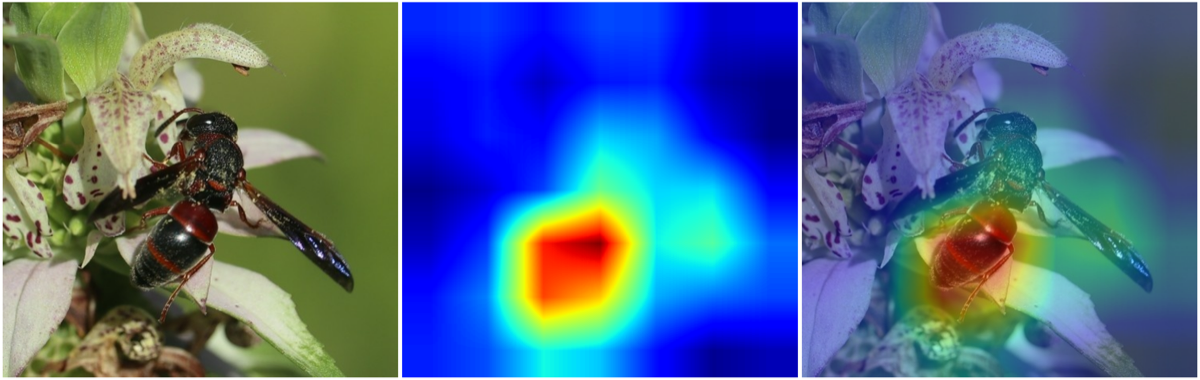
\includegraphics[width=\linewidth]{image/grad_cam/gradcam_correct_1.png}
    \caption{Correct Sample 1: \textit{Pachodynerus erynnis} (Wasp, Top-1 Prob: 0.8703). High activation on abdomen and thorax.}
    \label{fig:correct_1}
  \end{subfigure}
  \hfill
  \begin{subfigure}{0.48\textwidth}
    \centering
    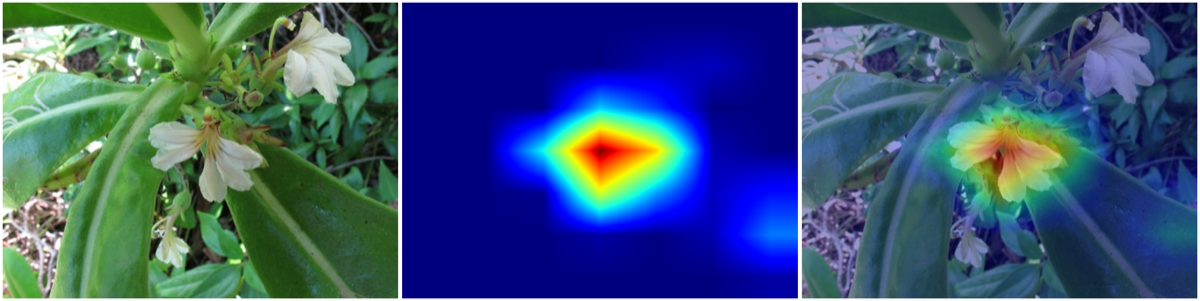
\includegraphics[width=\linewidth]{image/grad_cam/gradcam_correct_2.png}
    \caption{Correct Sample 2: \textit{Scaevola taccada} (Beach Cabbage, Top-1 Prob: 0.1133). Focus on petal fan structure.}
    \label{fig:correct_2}
  \end{subfigure}

  \vspace{0.4em}

  \begin{subfigure}{0.48\textwidth}
    \centering
    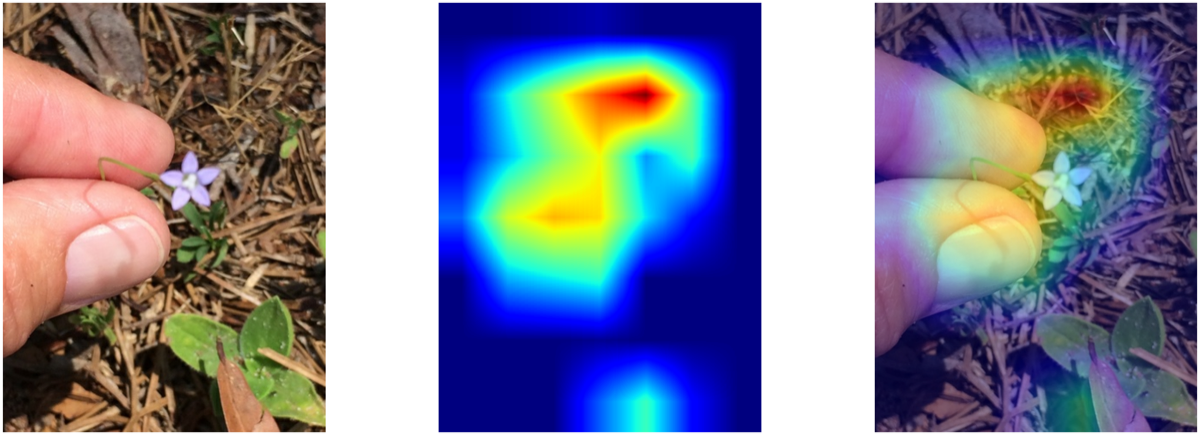
\includegraphics[width=\linewidth]{image/grad_cam/gradcam_incorrect_1.png}
    \caption{Failure Case 1: Ground-truth \textit{Wahlenbergia marginata} misclassified as near-relative \textit{W. albomarginata} (Prob: 0.0356).}
    \label{fig:incorrect_1}
  \end{subfigure}
  \hfill
  \begin{subfigure}{0.48\textwidth}
    \centering
    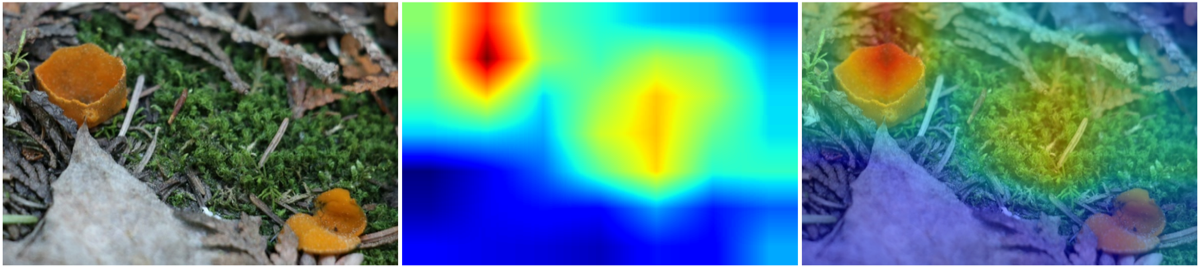
\includegraphics[width=\linewidth]{image/grad_cam/gradcam_incorrect_2.png}
    \caption{Failure Case 2: Ground-truth cup fungus \textit{Caloscypha fulgens} misclassified as lichen \textit{Peltigera membranacea} (Prob: 0.0310).}
    \label{fig:incorrect_2}
  \end{subfigure}
  \caption{\textbf{Grad-CAM visual explanations for correct predictions and failure cases.} Top row (\cref{fig:correct_1,fig:correct_2}): Correctly classified samples showing high activation (red/yellow) conforming tightly to morphological boundaries (abdomen, thorax, petals). Bottom row (\cref{fig:incorrect_1,fig:incorrect_2}): Misclassified samples illustrating fine-grained intra-genus ambiguity and complex forest-floor background distraction.}
  \label{fig:gradcam_overview}
  \label{fig:gradcam_correct}
  \label{fig:gradcam_incorrect}
\end{figure*}

\subsubsection{Part 1: Correct Predictions (Semantic Feature Localization)}
\label{sec:part1-correct}

To verify whether the fine-tuned ConvNeXt V2 model relies on genuine biological morphology rather than background artifacts, we inspect activation heatmaps for randomly sampled correctly classified test images (\cref{fig:gradcam_correct}).

As illustrated in \cref{fig:gradcam_correct}, for \textit{Pachodynerus erynnis} (\cref{fig:correct_1}), the peak activation hotspot (red/yellow) is tightly concentrated along the red-and-black abdominal segments and thoracic thorax. Similarly, for \textit{Scaevola taccada} (\cref{fig:correct_2}), the network highlights the distinctive fan-shaped white petals and glossy leaf cluster. This confirms that the model has learned meaningful anatomical features rather than exploiting background foliage shortcuts.

%-------------------------------------------------------------------------
\subsubsection{Part 2: Failure Cases (Incorrect Predictions Diagnostic)}
\label{sec:part2-incorrect}

Understanding misclassifications is essential for identifying model vulnerabilities. \cref{fig:gradcam_incorrect} presents Grad-CAM visual explanations for failure cases where top-1 predictions diverged from ground-truth labels.

Our diagnostic analysis of \cref{fig:gradcam_incorrect} reveals two primary failure modes:
\begin{enumerate}
  \item \textbf{Fine-Grained Intra-Genus Ambiguity}: In \cref{fig:incorrect_1}, the ground-truth specimen is \textit{Wahlenbergia marginata} (Southern Bluebell), but the model predicted its sister species \textit{Wahlenbergia albomarginata}. The model correctly localized the flower genus, but extreme visual overlap between floral petals under outdoor glare caused confusion between species within the same genus.
  \item \textbf{Habitat Forest-Floor Distraction}: In \cref{fig:incorrect_2}, the target \textit{Caloscypha fulgens} (a small cup fungus) is surrounded by dense forest moss and leaf litter. Gradient energy misdirected onto background moss textures rather than the small fungal fruiting body, resulting in misclassification as lichen.
\end{enumerate}

%-------------------------------------------------------------------------
\subsubsection{Part 3: Confusable Species Pairs (Fine-Grained Discrimination)}
\label{sec:part3-confusable}

A key challenge in biodiversity monitoring is discriminating morphologically similar species from the same genus. We evaluate Grad-CAM across three confusable pairs selected via randomized image sampling across distinct biological classes: Spiders (\textit{Steatoda}), Bumblebees (\textit{Bombus}), and Mint Moths (\textit{Pyrausta}). As illustrated in the supplementary material (\cref{sec:suppl-gradcam-confusable}, \cref{fig:suppl-gradcam-confusable}), ConvNeXt V2 correctly classifies all six species instances across the three confusable pairs:
\begin{itemize}
  \item \textbf{Genus \textit{Steatoda}}: For \textit{S. capensis} vs.\ \textit{S. grossa}, the detection primarily targets the body and head, while extending to include the spider's legs for both images, which indicate that the model can classify similar-looking but different species according to their morphological and anatomical features.
  \item \textbf{Genus \textit{Bombus}}: For \textit{B. huntii} vs.\ \textit{B. mixtus}, the attention on the first image is drawn mainly on the head of the bee, while the second image targets not only on its head but also several parts of the body.
        Notably, due to the noise background in the first image, the attention was also drawn by the flowers surrounded, as we can tell from the heatmap.
  \item \textbf{Genus \textit{Pyrausta}}: For \textit{P. purpuralis} vs.\ \textit{P. aurata}, activation maps isolate vibrant purple-gold wing patterns on \textit{P. purpuralis} and central golden-yellow forewing spots on \textit{P. aurata}, demonstrating fine-grained anatomical discrimination across distinct insect groups.
\end{itemize}

%-------------------------------------------------------------------------
%-------------------------------------------------------------------------
\subsection{Image Degradation Robustness Evaluation}
\label{sec:robustness-eval}

\begin{figure*}[t]
  \centering
  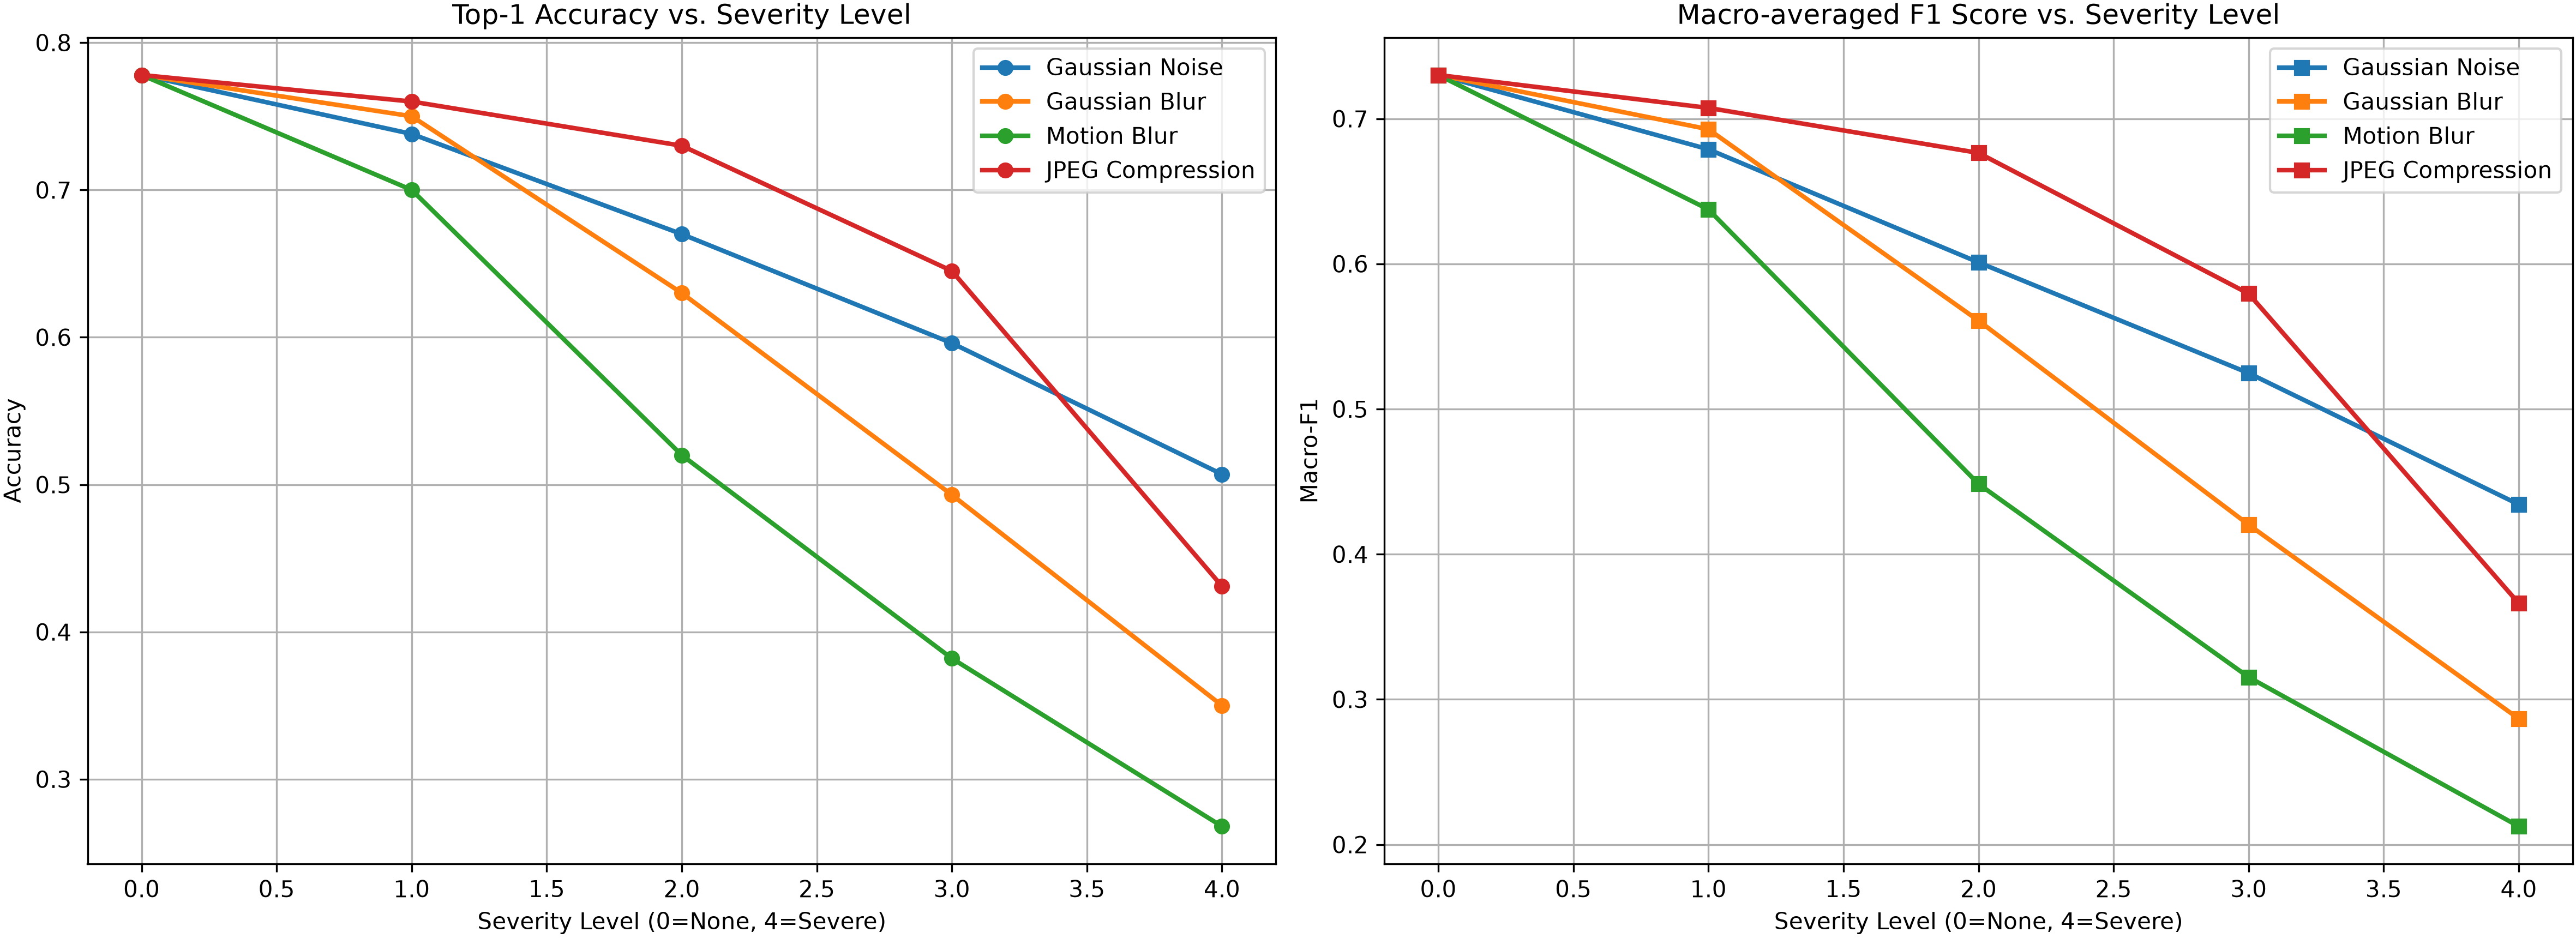
\includegraphics[width=0.82\linewidth]{image/robustness_analysis/robustness_curves.png}
  \caption{\textbf{Performance-versus-severity curves across 1,000 species under 4 image degradation types.} Left: Top-1 Accuracy vs.\ Severity Level ($0 = \text{Clean}$, $4 = \text{Severe}$). Right: Macro-averaged F1 Score vs.\ Severity Level. Baseline uncorrupted images achieve $77.80\%$ Top-1 Accuracy and $73.01\%$ Macro F1.}
  \label{fig:robustness_curves}
\end{figure*}

We evaluate the fine-tuned ConvNeXt V2 model across all 1,000 fine-grained species classes under synthetic image quality corruptions across 5 severity levels ($s \in [0, 4]$) as specified in \cref{sec:robustness-method}. \cref{fig:robustness_curves} plots the resulting Top-1 Accuracy and Macro-averaged F1 Score performance curves.

On uncorrupted clean images ($s=0$), the model achieves a baseline Top-1 Accuracy of \textbf{77.80\%} and a Macro F1 score of \textbf{73.01\%}. As demonstrated in \cref{fig:robustness_curves}, performance degrades monotonically across all 4 degradation types, revealing distinct levels of architectural sensitivity:

\begin{itemize}
  \item \textbf{JPEG Compression (Highest Resilience)}: ConvNeXt V2 exhibits exceptional tolerance to compression artifacts. At Level 1 ($q=50$) and Level 2 ($q=25$), Top-1 accuracy remains high at $76.00\%$ and $73.00\%$ respectively. Even under heavy compression at Level 3 ($q=10$), the model retains $64.50\%$ accuracy ($57.95\%$ Macro F1), before dropping to $43.10\%$ at extreme compression ($q=5$). This demonstrates that deep convolutional feature maps are robust to high-frequency $8 \times 8$ DCT block quantization noise.

  \item \textbf{Additive Gaussian Noise (Moderate Linear Degradation)}: Adding Gaussian pixel noise leads to a steady, nearly linear decline in accuracy, moving from $73.80\%$ at Level 1 ($\sigma=0.05$) to $50.70\%$ at Level 4 ($\sigma=0.20$, Macro F1 of $43.43\%$). Because depthwise $7 \times 7$ convolutions aggregate local spatial context, the network filters out moderate pixel-level variance better than fine blur.

  \item \textbf{Gaussian Blur (Steep Defocus Decay)}: Defocusing induces sharper degradation than noise. While mild blur ($r=1.0$) retains $75.00\%$ accuracy, performance drops to $63.00\%$ at Level 2 ($r=2.0$) and degrades heavily to $35.00\%$ at Level 4 ($r=4.0$, Macro F1 of $28.67\%$). Spatial smoothing erodes high-frequency edge gradients required for fine-grained morphological identification.

  \item \textbf{Motion Blur (Most Destructive Distortion)}: Directional motion streak convolution causes the steepest performance collapse, with accuracy dropping from $70.00\%$ at Level 1 ($L=5$) down to $52.00\%$ at Level 2 ($L=9$) and reaching a low of \textbf{26.80\%} at Level 4 ($L=17$, Macro F1 of $21.25\%$). Because motion blur smears diagnostic biological structures (\eg, insect leg segments, wing veins, and floral stamen) along a diagonal trajectory, local depthwise spatial kernels fail to extract discriminative cues.
\end{itemize}
